\documentclass{beamer}

\usepackage{graphicx}
\usepackage[utf8]{inputenc}
\usepackage[T1]{fontenc}
\usepackage{lmodern}
\usepackage[english]{babel}
\usepackage{amsmath}
\usepackage{amsthm}
\usepackage{mathtools}
\usepackage{amssymb}
\usepackage{listings}
\usepackage{xparse}
\usepackage{geometry}
\usepackage{enumerate}
\usepackage{tikz}
\usepackage{stmaryrd}
\usepackage[style=english]{csquotes}
\usepackage[language=english, backend=biber, style=alphabetic, sorting=nyt]{biblatex}

\usetikzlibrary{babel, positioning, shapes.geometric, arrows, arrows.meta}
\addbibresource{bibliography.bib}

\title{Generating random supersingular Elliptic Curves using modular polynomials}
\author{Simon Pohmann\\Supervisor: Cristophe Petit}

\newcommand{\N}{\mathbb{N}}
\newcommand{\Z}{\mathbb{Z}}
\newcommand{\F}{\mathbb{F}}
\newcommand{\C}{\mathbb{C}}
\newcommand{\I}{\mathbb{I}}
\newcommand{\V}{\mathbb{V}}
\newcommand{\End}{\mathrm{End}}
\newcommand{\proj}{\mathrm{proj}}
\newcommand{\Quot}{\mathrm{Quot}}
\newcommand{\Half}{\mathcal{H}}
\newcommand{\Lattice}{\mathcal{L}}
\newcommand{\divides}{\ \mid \ }
\newcommand{\notdivides}{\ \nmid \ }
\newcommand{\Cl}{\mathrm{Cl}}
\renewcommand{\a}{\mathfrak{a}}
\renewcommand{\b}{\mathfrak{b}}
\renewcommand{\O}{\mathcal{O}}
\renewcommand{\N}{\mathfrak{N}}

\newcommand\restr[2]{{
    \left.\kern-\nulldelimiterspace
    #1
    \vphantom{\big|}
    \right|_{#2}
}}

\newtheorem{proposition}{Proposition}
\newtheorem{question}{Question}

\begin{document}

\maketitle

\section{Fundamentals}

\begin{frame}
    \frametitle{Elliptic Curves}
    \begin{definition}
        An \emph{Elliptic Curve} is a projective variety with a defining equation of the form
        \begin{equation*}
            y^2 z = x^3 + Ax z^2 + B z^3
        \end{equation*}
    \end{definition}
    \begin{itemize}[<+->]
        \item Affine points of $E$ are $(x, y) \in \bar{k}^2$ such that $y^2 = x^3 + Ax + B$
        \item One point ``at infinity''
        \item $E$ defined over field $k$ if $A, B \in k$
    \end{itemize}
\end{frame}

\begin{frame}
    \frametitle{Elliptic Curves are groups}

    \begin{proposition}
        Let $E$ be an Elliptic Curve over $k$.
        Then there is $+_E: E \times E \to E$ such that $E$ becomes a group.

        Further, $+_E$ is (locally) given by polynomials.
    \end{proposition}
    \begin{itemize}[<+->]
        \item $E$ is an \emph{algebraic group}
        \item For $x_1 \neq x_2$, define $(x_1, y_1) +_E (x_2, y_2)$ to be
        \begin{align*}
            &\Bigl( \Bigl(\frac {y_2 - y_1} {x_2 - x_1}\Bigr)^2 - x_1 - x_2, \ (2x_1 + x_2)\frac {y_2 - y_1} {x_2 - x_1} - \Bigl(\frac {y_2 - y_1} {x_2 - x_1}\Bigr)^3 - y_1 \Bigr)
        \end{align*}
    \end{itemize}
\end{frame}

\begin{frame}
    \frametitle{Isogenies}

    \begin{definition}
        An algebraic map (i.e. morphism) between Elliptic Curves $E \to E'$ is called isogeny, if it maps $\infty \mapsto \infty$.
    \end{definition}
    \begin{itemize}[<+->]
        \item ``algebraic map'' $=$ ``locally given by polynomials''
        \item isogenies are automatically group homomorphisms
        \item important subclass: \emph{separable} isogenies
        \item 1-1 correspondence
        \begin{align*}
            \text{separable isogenies $E \to E'$} \ &\leftrightarrow \ \text{subgroups $G \leq E$} \\
            \phi \ &\mapsto \ \ker(\phi)
        \end{align*}
        \item degree of separable isogeny is $\#\ker(\phi)$
        \item $l$-isogeny $:=$ degree $l$ isogeny
    \end{itemize}
\end{frame}

\begin{frame}
    \frametitle{Isogenies (continued)}
    
    \begin{definition}
        An algebraic map (i.e. morphism) between Elliptic Curves $E \to E'$ is called isogeny, if it maps $\O \mapsto \O$.
    \end{definition}

    \begin{itemize}[<+->]
        \item Group law given by polynomials
        \begin{equation*}
            \text{$\Rightarrow$ have isogeny} \quad [m]: E \to E, \quad P \mapsto \underbrace{P + ... + P}_{\text{$m$ times}}
        \end{equation*}
        \item If $E$ defined over $\F_q$
        \begin{equation*}
            \text{$\Rightarrow$ have isogeny} \quad \pi: E \to E, \quad (x, y) \mapsto (x^q, y^q)
        \end{equation*}
    \end{itemize}
\end{frame}

\section{Isogeny graphs and crypto}

\begin{frame}
    \frametitle{Supersingular and ordinary curves}
    The endomorphisms (isogenies $E \to E$) of $E$ form a ring $\End(E)$.
    \begin{itemize}
        \item $\Z \hookrightarrow \End(E)$ as $[m]$ is isogeny
    \end{itemize}
    \pause
    \begin{proposition}
        If $k = \F_q$ is a finite field, then one of the following holds
        \begin{itemize}
            \item $\End(E)$ is an order in a quadratic imaginary number field
            \item $\End(E)$ is an order in a quaternion algebra
        \end{itemize}
    \end{proposition}
    \pause
    \begin{definition}
        In the first case, $E$ is called \emph{ordinary}, otherwise \emph{supersingular}.
    \end{definition}
\end{frame}

\begin{frame}
    \frametitle{Isogeny graphs}
    Elliptic Curves up to isomorphism are classified by \emph{j-invariant} $j(E)$
    \begin{itemize}[<+->]
        \item $l$-isogeny graph: \begin{minipage}[t]{0.6\textwidth}
            $V = \{ j(E) \ | \ \text{$E$ defined over $\F_q$} \}$\\
            $E = \{ (j(E), j(E') \ | \ \text{$\exists$ $l$-isogeny $E \to E'$}) \}$
        \end{minipage}
        \item The supersingular $l$-isogeny graph is an expander
        \begin{itemize}
            \item Useful for cryptography
        \end{itemize}
        \item Ordinary $l$-isogeny graphs are ``vulcanoes''
    \end{itemize}
    \visible<2->{\begin{minipage}{0.49\textwidth}
        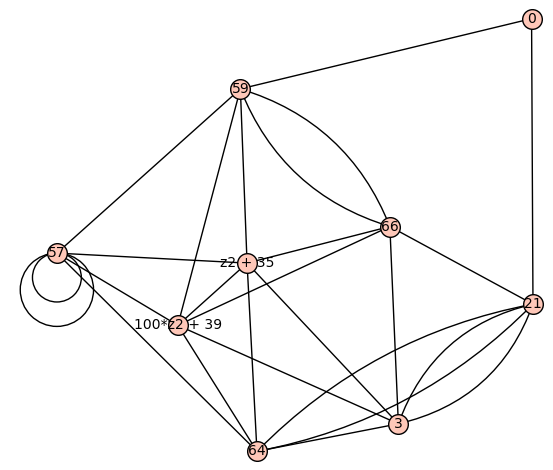
\includegraphics[width = \textwidth]{./example_supersingular.png}
    \end{minipage}}
    \visible<4->{\begin{minipage}{0.49\textwidth}
        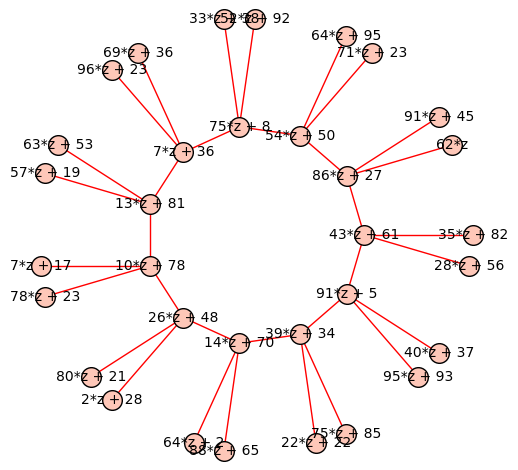
\includegraphics[width = \textwidth]{./example_odd_crater.png}
    \end{minipage}}
\end{frame}

\begin{frame}
    \frametitle{Generating supersingular curves}

    \begin{itemize}
        \item Classical approach: Random walk in isogeny graph
    \end{itemize}
    \pause
    \begin{question}
        Is there a method that does not reveal a path to a fixed curve?
    \end{question}
    \pause
    \begin{itemize}
        \item Experiments have shown correlation between supersingularity and having (multiple) $l$-isogenies $E \to E^{(p)}$, for fixed $l$.
        \begin{itemize}
            \item First explored in \cite{base_paper}, with limited success
        \end{itemize}
    \end{itemize}
    \pause
    \begin{question}
        How many ordinary resp. supersingular curves with $l$-isogeny $E \to E^{(p)}$ exist?
    \end{question}
\end{frame}

\begin{frame}
    \frametitle{Modular Polynomials}

    \begin{proposition}
        There is a polynomial $\Phi_l(x, y) \in \Z[x, y]$ such that $\Phi_l(j(E), j(E')) = 0$ if and only if there is an $l$-isogeny $E \to E'$.
    \end{proposition}
    \pause
    \begin{itemize}[<+->]
        \item Finding a curve with $l$-isogeny $E \to E^{(p)}$ is as easy/as hard as finding a root of $\Phi_l(x, x^p)$
        \item Finding a curve with an $l_1$-and an $l_2$ isogeny $E \to E^{(p)}$ corresponds to finding a root of $\mathrm{gcd}(\Phi_{l_1}(x, x^p), \Phi_{l_2}(x, x^p))$
    \end{itemize}
    \pause
    \begin{question}
        Is there a way to find a root of $\mathrm{gcd}(\Phi_{l_1}(x, x^p), \Phi_{l_2}(x, x^p))$ for exponentially large $l_1, l_2$ (and of course $p$)?
    \end{question}
\end{frame}

\begin{frame}
    \begin{center}
        \Huge
        Thank you for your attention!
    \end{center}
    \printbibliography
\end{frame}

\end{document}